\documentclass[twoside,12pt]{cslreport}

\usepackage{alltt,times,url,cite}
\usepackage{amsfonts,latexsym,amssymb}
\usepackage{graphicx}
\usepackage{listings}

\newenvironment{prtty_prg}{\begin{center}\begin{minipage}{\textwidth}\begin{tabbing}}
	 		  {\end{tabbing}\end{minipage}\end{center}}

\newcommand{\res}[1]{{\bf #1}}
\newcommand{\procedure}{\res{proc}\=\res{edure}\ }
\newcommand{\foreach}{\res{for }\=\res{each}\ }
\newcommand{\while}{\res{wh}\=\res{ile}\ }
\newcommand{\ploop}{\res{loop}\=\ }
\newcommand{\process}{\res{proc}\=\res{ess}\ }

\newcommand{\N}{\mbox{${\cal N}$}}
\newcommand{\B}{\mbox{${\cal B}$}}
\newcommand{\F}{\mbox{${\cal F}$}}
\renewcommand{\L}{\mbox{${\cal L}$}}
\newcommand{\U}{\mbox{${\cal U}$}}
\renewcommand{\S}{\mbox{${\cal S}$}}
\newcommand{\X}{\mbox{${\cal X}$}}
\newcommand{\dupdate}{\triangleleft}

%% \newcommand{\Q}{\mbox{$I\:\!\!\!\!\!Q$}}           % rationals
\newcommand{\Q}{\rational}


\newcounter{proglineno}

\newcommand{\putno}{\refstepcounter{proglineno}\begin{scriptsize}\textcolor{cyan}{\arabic{proglineno}:}\end{scriptsize}~}

\lstset{language=C,
  basicstyle=\fontfamily{pcr}\selectfont\footnotesize\color{black},
  keywordstyle=\color{black}\bfseries, % style for keywords
  %morekeywords=sassert,
  %morekeywords=malloc,
  numbers=none, % where to put the line-numbers
  % the size of the fonts that are used for the line-numbers
  numberstyle=\tiny,
  %backgroundcolor=\color{codebg},
  showspaces=false, % show spaces adding particular underscores
  showstringspaces=false, % underline spaces within strings
  showtabs=false, % show tabs within strings adding particular underscores
  %frame=single, % adds a frame around the code
  %tabsize=2, % sets default tabsize to 2 spaces
  %rulesepcolor=\color{gray},
  %rulecolor=\color{black},
  moredelim=[s]'',
  captionpos=b, % sets the caption-position to bottom
  breaklines=true, % sets automatic line breaking
  breakatwhitespace=false}

\lstnewenvironment{clisting}{\lstset{language=C,basicstyle=\ttfamily\scriptsize}}{}

\lstnewenvironment{cpluslisting}{\lstset{language=C++,basicstyle=\ttfamily\scriptsize}}{}




\addtolength{\oddsidemargin}{-4mm}
\addtolength{\topmargin}{-4mm}
\addtolength{\textwidth}{8mm}
\addtolength{\textheight}{8mm}

\newcommand{\real}{\ensuremath{\mathbb{R}}}
\newcommand{\nat}{\ensuremath{\mathbb{N}}}
\newcommand{\integer}{\ensuremath{\mathbb{Z}}}
\newcommand{\rational}{\ensuremath{\mathbb{Q}}}

\title{{\bf Where Art Thou Heap Metadata?}\\[5mm]
\Large  DARPA Contract Number N66001-15-C-4061\\[5mm] 
Final Report}

\author{Ian A. Mason (PI), Drew Dean, Bruno Dutertre,\\
  Jorge A. Navas, and Dan Wallach}

\begin{document}

\pagestyle{plain}

\maketitle

\cleardoublepage
\tableofcontents
\listoffigures
\listoftables

\cleardoublepage


%%%%%%%%%%%%%%%%%%%%%%%%%%%%%%%%%%%%%%%
\chapter{Introduction}
%%%%%%%%%%%%%%%%%%%%%%%%%%%%%%%%%%%%%%%

This document summarizes the research performed under DARPA Contract
Number N66001-15-C-4061 by SRI International, and presents the
project's results. The project started in August 2015 and was
completed in August 2017. The Principal Investigator for this project
was Drew Dean, until his departure in July 2016. Ian A. Mason took
over as PI after Drew Dean left. The co-investigators were Bruno
Dutertre (SRI), Jorge Navas (SRI), and Dan Wallach (Rice University).


%%%%============================
\section{Project Overview}
%%%%============================

Almost all modern programs make extensive use of dynamically allocated
data structures  such as  linked lists, trees,  and other  pointer- or
reference-filled data structures. If the  lifetime of the data exceeds
the lifetime  of the  function or  method allocating  the data,  as is
often the case, then  the data can not be allocated  on the stack, and
is  instead allocated  from the  heap.\footnote{There are  conflicting
  uses of  the word ``heap'' as  a heap is  also the name of  a specific
  data structure. We  use the computer science  systems terminology in
  this white  paper, where  a process' address  space is  divided into
  sections commonly  referred to as  code (aka text), data,  heap, and
  stack  space.}  Dynamically  allocated data  structures are  popular
because they allow programs not to have hard-coded limits in them, and
adapt their memory use to the actual usage of the program, rather than
a  developer's best  guess as  to how  the application  will be  used.

There  are  two  primary   downsides  to  dynamically  allocated  data
structures:
\begin{enumerate}
\item Na\"{\i}ve use  of  dynamic  memory allocation  can  incur
significant  performance  cost.
\item Pointer usage errors can introduce additional security
  vulnerabilities into software, particularly a class of vulnerability
  known as a heap overflow.  
\end{enumerate}

This project investigates backward-compatible improvements to dynamic
memory allocation that mitigate the security vulnerabilities of
dynamically allocated data structures.

\section{Background}


We focus on applications written in C that use the system provided
\texttt{malloc()} and \texttt{free()} routines.\footnote{For
  simplicity of discussion, we omit \texttt{calloc()},
  \texttt{realloc()}, \texttt{valloc()}, and
  \texttt{posix\_memalign()}, and the default \texttt{C++}
  \texttt{new} and \texttt{delete} operators. These pose the exact
  same issues and are covered by our approach.}  As expected, the use
of dynamically allocated data structures incurs some overhead; in
particular, \texttt{malloc()} and \texttt{free()} need to manage heap
space, keeping track of what memory is currently in use, and what
memory is currently free and available.  We call this overhead
\emph{malloc metadata\/}, as there is no standard terminology.  The
traditional place to store malloc metadata is in the heap itself, and the most troublesome
heap overflow exploits take advantage of this placement.\footnote{Pointer misuses can introduce
  arbitrary bugs and vulnerabilities into software, but overwriting of
  malloc metadata is the predominant exploitation vector of heap
  overflow vulnerabilities.} Figure~\ref{heap-example} shows a
simple visualization of the heap.  The important point is that the
dynamically allocated data and malloc metadata are contiguous and
interspersed. The color of any given heap location may change over
time, as memory is allocated and returned to the heap.  The
\texttt{free()} routine, however, implicitly assumes that addresses it
expects to be red, are actually red. Given certain pointer errors
(such as the double freeing of a pointer), an attacker can violate
this assumption, which can lead to arbitrary code execution.  An
illustrative example can be found in CERT Advisory CA-2002-07,
``Double Free Bug in zlib Compression Library.'' Regrettably little
progress has been made in the intervening 13 years, as this
vulnerability has been repeated over and over.

\begin{figure}
\begin{center}

\includegraphics{heap-example}
\end{center}
\caption[Schematic Layout of a Standard Heap]{Schematic Layout of a
  Standard Heap. Malloc metadata is in red, dynamically-allocated data
  structures are in black, and free memory is in white. Both red and
  black areas have pointers to same-colored addresses. A real heap
  would have thousands/millions regions of red and black.}
\label{heap-example}
\end{figure}


\section{Approach}

We propose to refactor the implementation of \texttt{malloc()} and
\texttt{free()} to produce a heap layout as shown in
Figure~\ref{heap-split}.  The important difference is that the
malloc metadata is held in a separate memory region, one that is not
contiguous with the heap. This metadata region is allocated by the operating
system at a randomized address, and so its location cannot be deduced from the
address of the client memory.

This separation improves security, but its implementation requires a
mechanism for locating the metadata associated with a particular
client memory address.  Implementing this {\em lookup mechanism\/}
efficiently---especially in a multi-threaded situation---is the core
problem we face in this project.

In the single-threaded case, a hash table is an efficient data
structure that adds minimal overhead to finding the metadata
associated with a dynamically allocated pointer. This prevents
simple errors from corrupting malloc metadata.  Instead of reallocated
heap data getting confused with malloc metadata (as in CERT-2002-07),
an attacker would need primitives to both read the pointer to this
region, and overwrite arbitrary memory locations. While such attack
primitives are certainly possible, the attacker's workload has been
increased, and the current stockpile of heap overflow vulnerabilities
become obsolete.  A side benefit of our approach is that a double free
bug can be readily detected and ignored or logged for debugging
purposes.  In an ideal world, the malloc metadata would be stored in a
separate protection domain.  In the CHERI architecture developed by
SRI and Cambridge University in DARPA's CRASH program, this would be
easy to implement efficiently with capabilities. Conventional machines
would need to use another process to guarantee separation, which may
impose too much overhead, depending on the performance of interprocess
communication mechanisms.

\begin{figure}
\begin{center}

\includegraphics{heap-split}
\end{center}
\caption[Schematic Heap with Separate Metadata]{Schematic Heap with
  Separate Metadata. Color codes are as in Fig.~\ref{heap-example}.}
\label{heap-split}
\end{figure}


\section{Accomplishments}

In  year  one  of  this   project,  we  produced  several  prototypes,
culminating with an  alpha version of a variant of  glibc's malloc for
x86-64  Linux  called  \texttt{sri-glibc}.  This  allocator  does  not
include any metadata in client memory.  It is {\em thread safe\/}, and
introduces no new  contention compared to the  glibc original. Ongoing
benchmarking indicates that the overhead  is often very much less than
10\%.   One  of  the  key  ingredients  to  \texttt{sri-glibc}  is  an
efficient lock-free mechanism that maps  client addresses to the arena
the memory belongs to.

In year two, we focused on verification and re-implementation of our
hash table. The version we developed in year one had several
concurrency bugs that we fixed in year two. In addition, we have
addressed a significant issue related to memory management. Our hash
tables rely on linear probing and expand when the current capacity is
insufficient. This creates larger and larger copies of the table. Old
copies eventually become inaccessible and not touched by any
thread. Our year-one implementation did not keep track of this and
never released any copy. The new implementation detects when old
copies are no longer necessary and releases the corresponding memory
to the operating system. We have developed our new hash-table
implementation as a stand-alone package, independent of malloc.

We have also formalized key aspects of the hash-table implementation,
namely the growing and data migration mechanism. We have developed a
state-machine model of these mechanisms and verified critical
properties using the SAL model checker.


\section{Publications}

The following paper describes improvements to the SeaHorn static
analyzer that were developed as part of this project, in an attempt to
prove the absence of null pointer dereferences in openBSD's malloc:
\begin{quote}
  Arie Gurfinkel and Jorge A. Navas, A Context-Sensitive Memory Model
  for Verification of C/C++ Programs, {\em Static Analysis Symposium
    (SAS~2017)\/}.
\end{quote}
This paper will be presented at the 24th Static Analysis Symposium
to be held in New York City from August 30th to September 1st, 2017.


\section{Software}

We have developed several prototypes of malloc and lock-free hash
tables during the project. Our re-implementation of GNU Libc's malloc
that separates metadata from the head is publicly available under an
open-source license at~\url{https://github.com/SRI-CSL/sri-glibc-malloc}.




%%%============================================
\chapter{Summary of Research and Results}
%%%============================================

The main results of this project are prototype implementations of
malloc libraries, and implementations of lock-free hash tables. We
also applied verification tools including static analyzers and model
checkers to these software implementation and algorithms.

\section{Family Tree of Glibc Allocators}
\label{family-tree}

Most of the malloc prototypes we developed belong to the family of
memory allocators commonly used with Linux, in particular the
Glibc-based distributions.  These include most Linux distributions
that do not target embedded systems. Figure~\ref{fig:tree} gives an
abridged family tree of these memory allocators.

The root of the tree is Doug Lea's malloc (\texttt{dlmalloc}), which
was born in 1987.  It was originally intended for single threaded
applications with scarce resources.
%
Gloger's allocator (\texttt{ptmalloc2}) extends \texttt{dlmalloc} with
\emph{arenas}.  Arenas are independent self-contained heaps that can
be utilized simultaneously by separate threads, reducing contention
for global locks.
%
Glibc's built-in memory allocator is a direct descendent of
\texttt{ptmalloc2}. \texttt{Ptmalloc2}'s main attraction over Glibc
malloc is its ease of compilation. Glibc malloc is deeply entwined in
the Glibc infrastructure and is very difficult to extract into a
stand-alone library.  Glibc has also evolved somewhat since its fork
from \texttt{ptmalloc2}, the arena locking is somewhat more complex,
and the metadata has grown to include skip lists for the bin free
lists.

Piessens's \texttt{Dnmalloc}~\cite{YJP06} is a package from 2005 that modified
\texttt{dlmalloc} to move its metadata out of the heap, much like our
proposal. This implementation used a lookup table based on a 32 bit address
space that could not be extended to modern x86-64 hardware.


\begin{figure}[h]
\begin{center}
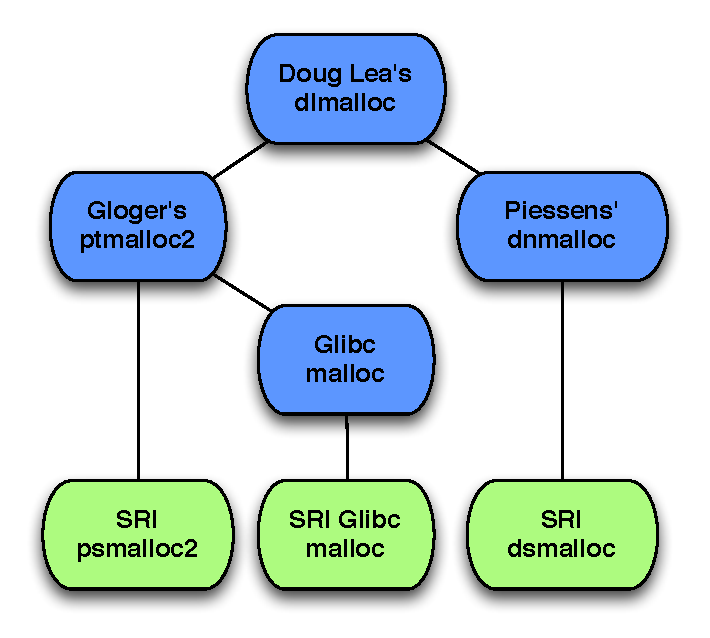
\includegraphics{OurFamilyTree.pdf}
\end{center}
\caption[The family tree of C memory allocators.]{The family tree of C
  memory allocators starting from Doug Lea's work in the 1990s. Blue
  allocators are ancestors of our work.  Green allocators have been
  developed within this project.}
\label{fig:tree}
\end{figure}


The green nodes in Figure~\ref{fig:tree} show three prototypes that we
developed in this project.
\begin{itemize}
\item Our first prototype (\texttt{dsmalloc}) generalized Doug Lea's
  malloc along the lines of \texttt{dnmalloc} by implementing linear
  hashing, a version of dynamic hashing that uses a variation of
  Larson's algorithm as published in~\cite{Larson:1988:DHT}.

\item Our second prototype (\texttt{psmalloc2}) builds upon Gloger's malloc (\texttt{ptmalloc2}).
\texttt{Psmalloc2} succeeds in removing almost all metadata from 
client memory. The only remaining piece of metadata is the index of the arena
the memory belongs to.
From a security point of view, what is critical is that the metadata
in the heap is an integer, not a pointer. If the integer is corrupted
(either by accident or by malice), \texttt{free()} or
\texttt{realloc()} won't be able to find the pointer, and can signal
an error, but these routines won't go chasing attacker supplied
pointers and end up overwriting security-critical data.
  
\item In our final prototype \texttt{sri-glibc}, we eliminated the need for
an arena number in the client chunk by implementing a lock-free API to
determine arena index from client pointer. We also tailored the
metadata to improve performance by reducing the number of hash table
lookups.  This \texttt{sri-glibc} prototype is an alpha version. We
tried to keep changes to a minimum, in the hope an upstream adoption,
however as the changes added up, a cleaner approach becomes more
apparent, and eventually essential.
\end{itemize}

In addition to the allocators mentioned previously---which all descend
from Doug Lea's malloc---we also examined malloc implementations in
Windows and Apple's OS~X and iOS. A summary of implementation and
security features is given in the Appendix.


\section{Lock-Free Data Structures}
\label{lock-free}

Because we separate metadata from client memory, all our prototypes
require a separate allocation mechanism for the metadata and the
related data structures. These are not full-fledged allocators since
they are dedicated to allocating objects of small range of (small)
sizes.  We call these {\em pool allocators\/}. To avoid excessive
overhead, we wanted our pool allocators to be lock-free. This led us
to Maged Michael's paper on scalable, lock-free dynamic memory
allocation~\cite{maged-michael-lfpa}.  This paper received PLDI's
``2004 Most Influential Paper Award'' in 2014.  The following quote
explains this award.
\begin{quote}
Maged Michael’s PLDI’04 paper is considered a landmark in memory
allocation for multi-threaded programs, presenting the first completely
lock-free general-purpose user-space allocator. It provides good
performance with respect to scalability, speed and space efficiency,
while at the same time only relying on common hardware and OS
support. The work is highly regarded and frequently referenced, and is
also the basis of multiple memory allocator implementations, both in
IBM products and in follow-on research.
\end{quote}

Working from a 32-bit x86 implementation of Michael's
algorithm~\cite{schneider-michael}, we have developed a 64-bit x86\_64
version (\texttt{elfpa}) that has no pointer metadata in the client memory. This is a
full malloc implementation that relies on an almost lock-free
hash table as a lookup mechanism.

Implementing a lock-free lookup was a major accomplishment of our
project that enabled us to remove all metadata from Glibc's malloc
library. This solved a key difficulty, namely, efficiently mapping an
arbitrary client pointer to the relevant arena without incurring the
cost of a locking contention.

In year one of the project, we implemented two versions of lock-free
dynamic hash table.  Both were influenced by Maier's
paper~\cite{maier-arxiv}.  Both implementations are based on linear
probing hash tables that expands when the current capacity is
insufficient. The most complex aspect of such tables is the expansion
phase. In one version, we relied on pthread locking and signaling
primitives to allow a single thread to grow the table. This prevents
concurrent access to the table while it is growing, which we
considered a tolerable tradeoff. This implementation could not be
ported to Glibc as the pthread primitives are not available. Instead,
we developed another growing mechanism that requires no locking. In
the growing phase, each thread that accesses the table must pay its
due by migrating key-value pairs from the old table to the new one.


In year two, we continued developing and improving the lock-free
dynamic hash table. We started a clean general-purpose version of the
table, independent of malloc. The overall design did not change. The
table maps 64~bit keys (i.e., integer or pointers) to 64~bit values.
We use linear probing and store the entries in a fixed-size
array. When this array is full, we create a new copy of double its
size and migrate data from the previous array to the new array. As
mentioned previously, this migration process is performed in a
decentralized fashions. Any thread that accesses the hash table must
first copy a fixed number of entries from the old to the new array.
We also improved the algorithm so that old array copies that are no
longer useful can be freed and the memory they use can be reclaimed by
the operating system. For this purpose, we rely on reference counting
to keep track of the number of threads that have a pointer to each
array copy. Properly managing and updating these reference counters
turned out to be quite difficult, and forced us to use locks in some
critical parts of the code to avoid race conditions. The new
implementation is then not entirely lock free. However, the locks are
used only in limited contexts during the migration process and
initialization of some data structures. In normal usage, operations
such as adding or removing entries, and searching for a key do not
require any locks. The appendix (Section~\ref{algorithm-details})
presents the hash-table design and algorithms in detail.

To get confidence in this hash-table implementation, we performed
extensive stress testing. We also applied formal verification to key
parts of the migration process.

%%% \section{Survey of Other Allocators}

\section{Formal Analysis}
\label{verification}

In year two of the project, we investigated several formal-method
tools and applied them to an existing malloc implementation and to our
own code, including our new dynamic hash table.

\subsection{Static Analysis of Malloc}

We have applied static analysis tools to a simplified version of
OpenBSD's memory allocation library. This library implements a
so-called BIBOP (Big Bag of Pages) allocation algorithm. This
allocator was implemented by Otto Moerbeek and was described at the
EuroBSD Conference in 2009~\cite{Moerbeek2009}. This allocator is an
interesting target for analysis since it is relatively simple and the
code is small, but the allocator achieves good performance.

In a first attempt, we applied the SeaHorn static
analyzer~\cite{Gurfinkel+etal:SeaHorn:2015} to this code, without any
modification. SeaHorn is an open-source verification tool for safety
properties of programs. It works at the level of LLVM bitcode so it
can be easily applied to software written in C or C++. SeaHorn can
check safety properties such as the absence of null-pointer
dereferences and buffer overflows. It can also verify user-provided
properties written as C-like assertions. Our initial goal was to show
that the OpenBSD malloc did not have null-pointer derefences.

It turned out that some of the algorithmic tricks used by OpenBSD were
beyond what can be modeled in SeaHorn, because the backend solver used
by SeaHorn works on problem formulated in linear arithmetic. The
OpenBDS code uses various bit-level encoding that do not translate to
linear arithmetic. As a result, analysis with SeaHorn does not work
well on the original code. The modeling to too imprecise and SeaHorn
produces to too many false positives.

We addressed these issues by replacing problematic parts of the code
with simpler variants (sometimes using non-deterministic constructs)
that are easier for SeaHorn to handle. We were able to prove the
absence of null-pointer dereferences for simple test drivers that
allocate constant-size chunks of memory. We then extended these
drivers to simulate an arbitrary number of calls to malloc immediately
followed by calls to free. Each malloc uses a non-deterministic size
argument. This test corresponds to the following loop:
\begin{lstlisting}[language=C]
    while (*) { sz = random(); p = malloc(sz); free(p); }
\end{lstlisting}
For this example, we did not obtain a complete proof with SeaHorn. The
tool did not find safe inductive invariants. But we could explore the
code using SeaHorn's bounded model checking engine after unrolling all
the loops eight times. We did not find any null pointer dereference.

A detailed analysis showed that the invariants necessary to prove the
absence of null-pointer dereference are beyond what the backend solver
can produce. For example, some of them require learning facts about
integer divisibility and other require quantifiers.

Overall, we found that automated verification of malloc algorithms
(even relatively simple ones) is beyond the reach of current static
analysis techniques. Semi-automated techniques where the code is
annotated by hand with invariants, pre-conditions, and post-conditions
might be applicable (e.g., using
FramaC~\cite{Kirchner+etal:FramaC:2015}). We did not have the resource
for such an exercise within the project.


\subsection{Modeling and Verification of Lock-Free Algorithms}

As an alternative to static analysis of code, we looked at
verification of higher-level, more abstract models of algorithms and
data structures. We focused on building state-machine models of some
of the lock-free algorithms we use and verifying invariant properties
using model checkers. We relied on the SAL and Sally model checkers.

SAL is a set of tools for specification and analysis of state
machines~\cite{deMoura+etal:SAL:2004}, developed and distributed by
SRI International. SAL includes traditional model-checking tools,
including a BDD-based symbolic model checker and bounded model
checkers for both finite and infinite systems. The state-machine
models we developed were all infinite and we analyzed them using pure
bounded model checking (to search for counterexamples to properties of
interest) and so-called $k$-induction. $K$-induction is a
generalization of the standard induction principle that can be used to
prove invariant properties of state-transition systems.  In most
cases, $k$-induction is not fully automated and requires the user to
discover useful auxiliary lemmas that can be proved by $k$-induction
and imply the property one cares about.

Our main results are based on a state-machine model of the data
migration algorithm used in our lock-free hash table. We proved a key
invariant of this algorithm using SAL. The proof involves a set of
auxiliary lemmas the we discovered and added by hand. Details of the
model and verification results are presented in the appendix.

We also experimented with SRI's new model checker called
Sally~\cite{Jovanovic+Dutertre:pdkind:2016}.  Sally is a more advanced
tool than SAL. It extends traditional $k$-induction with algorithms
that attempt to automatically discover an inductive strengthening of
the property of interest. Sally builds on the IC3 method due to
Bradley~\cite{bradley2011sat} and relies on SMT solvers to
incrementally discover relevant auxiliary lemmas. 

We attempted to verify the hash-table migration process using Sally,
starting with the same state-machine model we built for
SAL. Unfortunately, Sally does not manage to prove the key invariant
on its own. It learns larger and larger sets of auxiliary invariants
but it does not converge. This is a limitation of the underlying SMT
technology used by Sally. We believe that one of the auxiliary lemma
that we used in our manual proof with SAL is beyond what can be
learned automatically by Sally. In summary, the proof is too hard for
Sally to discover automatically. In future work, we will consider
alternative techniques for learning auxiliary invariants based on
abstract interpretation or other methods, which we believe might help
in this case.

Although Sally did not work on the most complex model we developed in
this project, we used it successfully to verify a simple
implementation of the CAS instruction, a non-blocking queue, and
Simpson's four-slot algorithm, a classical example of lock-free
algorithm for asynchronous communication~\cite{Simpson:four-slot:1990}.



\chapter{Conclusion}

We  have produced  several prototypes allocators, most of which were
derived from the glibc family tree, depicted in Figure~\ref{fig:tree}.
We also implemented Maged Michael's lock-free allocator, and a variety
of lock-free data structures.
This work culminates with an alpha version of a variant of  glibc's malloc for
x86-64  Linux  called  \texttt{sri-glibc}.
This  allocator  does  not
include any metadata in client memory.  It is {\em thread safe\/}, and
introduces no new  contention compared to the  glibc original. Ongoing
benchmarking indicates that the overhead  is often very much less than
10\%.   One  of  the  key  ingredients  to  \texttt{sri-glibc}  is  an
efficient lock-free mechanism that maps  client addresses to the arena
the memory belongs to.


%% In phase two of this project, we plan to improve the alpha version by 
%% completing the benchmarking, and refining the implementation details.
%% We also plan to open source all the software that we have developed in this
%% project. We will also broaden our approach from
%% just implementation to more formal methods.


%% As is well known, it is much easier to verify code designed for verification than to
%% verify existing code.
%% This is particularly true of the family of memory allocators rooted with Doug Lea's \texttt{dlmalloc}.
%% There is simply too much
%% complication in \texttt{dlmalloc} (e.g., the constantly
%% changing representations of a block depending on its current state)
%% for any realistic hope of formally verifying significant properties of
%% \texttt{dlmalloc}-family allocators in a small project.

%% As we wrap up
%% our work on removing heap metadata from the heap itself, we consider
%% what the next steps in securing the heap should be. The logical follow
%% on is to study the design space, investigating the formalization of
%% the relevant memory allocation algorithms and lock-free data
%% structures in order to analyze their properties and establish their
%% correctness in the context of a performant, realistic dynamic memory
%% allocator. While the full formal verification of a realistic, performant
%% dynamic memory allocator is beyond the scope of the proposed work,
%% this work will specify and implement an allocator amenable to
%% formal verification in future work.


%% We have three key desiderata:
%% \begin{enumerate}
%%   \item No metadata in front of client chunk,
%%     i.e. headerless chunks;
%%   \item  Progress in a memory allocation operation
%%     should not depend on a obtaining globally contended lock; 
%%   \item Amenable to verification/formal specification, or designed with
%%     that in mind. 
%% \end{enumerate}
%% No current memory allocator for C/C++ meets all
%% of these desiderata.

%% We plan to begin by experimenting with a prototype BIBOP
%% allocator, and conduct application level benchmarks (e.g., SPEC CPU 2006, Yices,
%% Cryptominisat, and a good multi-threaded application) to measure application
%% performance and memory use. With our experience as both users and
%% developers of formal verification tools (e.g., PVS, Yices, Sally) we
%% will also evaluate how tractable specification and verification of
%% different algorithms appear to be.  We will also use this time to fill
%% in any gaps that might remain in our understanding about the usability
%% of various lock-free data structures and algorithms from Phase 1. We
%% then proceed to the primary task of specifying and implementing our
%% chosen allocator design.




{\small
\bibliographystyle{plain} 
\bibliography{heap,malloc}
}


\appendix

%%%============================================
\chapter{Survey of Malloc Implementations}
%%%============================================

%% \subsection{Apple}

\section{Apple (OS X and iOS)}
Security researchers have paid attention to
Apple operating systems,~\cite{reverse}
but its memory allocator has received less attention.
Some discussion appears in Miller and
Zovi~\cite{mac-hackers-handbook-2009,ios-hackers-handbook-2012}
in 2009 and 2012.  The earliest public discussion seems to be from
Nemo~\cite{nemo2005} in 2005.

As of 2016, Apple uses two different \texttt{malloc} implementations:
\texttt{libmalloc} and \texttt{bmalloc}. \texttt{libmalloc} appears to date
from Apple's acquisition of NeXT, while \texttt{bmalloc} is a brand new
system, used in Apple's Safari browser. Both are distributed as open
source on Apple's web site\cite{libmalloc, bmalloc}. \texttt{bmalloc} is also distributed
as part of Apple's open source Webkit~\cite{webkit} (i.e., the open
source project from which Apple's Safari browser is derived).


\subsection{LibMalloc}
\label{sec:libmalloc}

\texttt{libmalloc} is implemented in C and exports a superset of the
usual \texttt{malloc} routines. Notably, it has a concept of {\em zones},
allowing a program to allocate fresh memory from any zone. Under the
hood, these zones are essentially the same as the {\em arenas} used in
the glibc memory allocators. With Apple
explicitly exposing these zones, a multi-threaded program can
explicitly manage multiple zones to avoid locking contention when
memory is allocated.

Zones also support {\em batch allocation}, facilitating
efficient  allocation of large numbers of objects of the same size.
Apple's developer pages promote these and other \texttt{libmalloc}-specific
features.\footnote{\url{https://developer.apple.com/library/mac/documentation/Performance/Conceptual/ManagingMemory/Articles/MemoryAlloc.html}}
Apple
also supports zone-specific allocation in its Cocoa Objective-C
libraries\footnote{\url{https://developer.apple.com/library/ios/documentation/General/Conceptual/CocoaEncyclopedia/ObjectAllocation/ObjectAllocation.html}}
and apparently zone allocation is also used inside the newer Swift
programming
environment.\footnote{\url{http://www.russbishop.net/swift-how-did-i-do-horrible-things}}

The downside of \texttt{libmalloc}'s approach, however, is that
alternative \texttt{malloc} implementations do not implement the various
zone-related methods and are not drop-in compatible with programs or
libraries that expect to have the extended \texttt{libmalloc} features.

\texttt{libmalloc} gives explicit credit to the Hoard allocator as an
influence on its design. This analysis focuses on management of the ``tiny''
regions, used for small object sizes.

Tiny objects are allocated from {\em regions}.
Each region is 1MB in
size and holds 64520 16-byte {\em blocks}.
A region also has a {\em region trailer} which contains the
metadata for the region.
The trailer includes a bitmask to track the free/busy
state of each tiny block. When a block is allocated, it has no
per-block header or trailer. Free blocks are maintained using a
doubly-linked list.

Apple's design, in the presence of a use-after-free situation,
potentially allows attackers to have access to the free-list
pointers. Furthermore, if an attacker can overflow the last block in a
region, the attacker will then have access to that region's metadata.

%% \begin{figure}
%% % \lstset{language="pascal",showstringspaces=false,basicstyle=\ttfamily}
%% % \begin{lstlisting}[frame=single]
%% \begin{description}
%% \item[MallocLogFile $<f>$] to create/append messages to file $<f>$ instead of stderr
%% \item[MallocGuardEdges] to add 2 guard pages for each large block
%% \item[MallocDoNotProtectPrelude] to disable protection (when previous flag set)
%% \item[MallocDoNotProtectPostlude] to disable protection (when previous flag set)
%% \item[MallocStackLogging] to record all stacks.  Tools like leaks can then be applied
%% \item[MallocStackLoggingNoCompact] to record all stacks.  Needed for
%%   {\sf malloc\_history}
%% \item[MallocStackLoggingDirectory] to set location of stack logs,
%%   which can grow large; default is {\sf /tmp}
%% \item[MallocScribble] to detect writing on free blocks and missing initializers: 0x55 is written upon free and 0xaa is written on allocation
%% \item[MallocCheckHeapStart $<n>$] to start checking the heap after $<n>$ operations
%% \item[MallocCheckHeapEach $<s>$] to repeat the checking of the heap after $<s>$ operations
%% \item[MallocCheckHeapSleep $<t>$] to sleep $<t>$ seconds on heap corruption
%% \item[MallocCheckHeapAbort $<b>$] to abort on heap corruption if $<b>$ is non-zero
%% \item[MallocCorruptionAbort] to abort on malloc errors, but not on out of memory for 32-bit processes. MallocCorruptionAbort is always set on 64-bit processes
%% \item[MallocErrorAbort] to abort on any malloc error, including out of memory
%% % \end{lstlisting}
%% \end{description}
%% \caption{Environment variables supported by {\sf libmalloc}.\label{fig:libmalloc-env}}
%% \end{figure}

\texttt{libmalloc} maintains a checksum in its heap metadata, added
sometime between 2009 and 2012, that defeats some heap metadata
overwrite attacks. A checksum is stored in the high four bits of
each free-list pointer, based on a randomly-generated
cookie~\cite{ios-hackers-handbook-2012}.

\texttt{libmalloc} also has a variety of flags that radically change how it
operates, along with a related {\em Guard Malloc}
library\footnote{\url{https://developer.apple.com/library/ios/documentation/Performance/Conceptual/ManagingMemory/Articles/MallocDebug.html}}. These help developers in
finding memory errors in their programs. They have a serious
impact upon performance. They could potentially be
repurposed for security if their performance could be
improved.
%% Figure~\ref{fig:libmalloc-env}
%% provides a list of the environment variables that control the security
%% checking.
Of note, \texttt{MallocGuardEdges} adds guard pages around large blocks, which will
cause memory overruns to abort. Also, several
environment variables instruct \texttt{libmalloc} to perform consistency
checks on its heap. If corruption is detected, the process will abort.

\subsection{BMalloc}
Before 2015, the Webkit browser used Google's \texttt{tcmalloc}, then
Apple abruptly replaced it with \texttt{bmalloc}. 

The \texttt{bmalloc} implementation does not
presently have the standard \texttt{malloc} API. Instead, a family of
similarly-named calls (``mbmalloc'', ``mbcalloc'', ``mbfree'', etc.)
are provided, along with an internal switch that can route these calls
to the ``real'' \texttt{malloc} implementation or handle them
internally. A program linked against \texttt{bmalloc} can then
be switched over to a third-party \texttt{malloc} implementation.
\texttt{bmalloc} does not expose anything
analogous to the ``zone'' features of \texttt{libmalloc}.

\texttt{bmalloc} has a unique design. It could be best described as ``lazy'', in that
when a block is freed, a pointer to it is placed in a fixed-size
buffer. In the common case, allocation and free operations are
constant time, with a very low cost.

\texttt{bmalloc} supports multiple {\em heaps}. A heap has {\em small
  pages} which in turn have {\em small lines}.
\texttt{bmalloc} tracks the free space within these small  lines.
Then, for each of a
variety of {\em size classes}, \texttt{bmalloc} maintains ``bump
allocators'' which are backed by those small lines. Objects are
allocated starting at the beginning of a line and continuing
sequentially to the end. 

Each heap has an asynchronous ``scavenger'' which processes its free lists,
looking for memory it can reuse. If the scavenger gets behind, the
normal allocation and memory freeing routines can also do the same
work.

Unlike \texttt{libmalloc}, memory objects in \texttt{bmalloc} never hold
metadata when they're freed. Instead of an inline free list, there is a
counter in the header for each line of memory to track how much is in
use versus how much is free. If the counter indicates a line of memory is
entirely unused, it can be recycled for future allocations.

The metadata resides in headers at the front of each heap. The
asynchronous nature of the free-list scavenger makes it harder for an attacker
to predict the state of the heap at any given time, which is otherwise
essential to Heap Feng Shui attacks.

\texttt{bmalloc} has no explicit features to detect 
use-after-free or double-free operations which might be exploited
as part of an attack, but it has clearly been engineered to make
some attacks more difficult.



%% \subsection{Windows}
\section{Windows}

Microsoft's Windows memory allocator has been the subject of regular
attention from the hacking community. In response, Microsoft has
developed particular security solutions for Internet Explorer and
legacy systems going back to Windows XP. As part of their ongoing
security efforts, Microsoft has also been improving the general resistance
of the default \texttt{malloc} implementation that ships with Windows.
Here, we focus particularly on the design in Windows 8.

\subsection{Browser-specific memory allocators}

Circa 2014, Internet Explorer introduced two new
defenses~\cite{yason2014,simonz2014}. 
\begin{description}
\item [Memory protector] Newly freed objects are zeroed out but are
  not immediately made available for reuse. Instead, a mark-and-sweep
  style system detects whether there are live references from the
  current call stack to any of these heap objects after they've been
  freed. This is effective at defeating ``use after free'' attacks.
\item [Isolated heap] This exposes multiple memory arenas to the
  user level, similar to Apple's \texttt{libmalloc} (see
  Section~\ref{sec:libmalloc}). Operations that could
  potentially cross arenas, like a \texttt{realloc}, will fail. This
  allows Internet Explorer to isolate potentially attackable objects (e.g., aspects
  of the HTML DOM) from system objects. This could help defeat some
  classes of heap overflow attacks.
\end{description}

In Windows 10, Microsoft rolled out ``MemGC'', which provides additional
memory protections for its Edge and Internet Explorer 10
browsers~\cite{yason2015}. MemGC provides a concurrent mark-and-sweep
garbage collector, which originates with Microsoft's JavaScript
implementation, but which also serves the rest of the browser runtime
system.

\subsection{Enhanced Mitigation Experience Toolkit}

Also in 2014, Microsoft released the fifth version of its Enhanced
Mitigation Experience Toolkit (EMET5)~\cite{metcalf2014}. EMET5 can be
applied to versions of Windows as old as Windows XP, and has a variety
of features, such as being able to prevent an application like Microsoft Word
from loading an Adobe Acrobat plugin. To hinder heap attacks,
EMET5 adds:
\begin{description}
\item [Heap spraying] Preallocates blocks in regions that known
  heap-spray attacks like to use. (Trivial for new attacks to work
  around.)
\item [Null page] The page at the bottom of memory is pre-allocated
  to defeat attacks meant to trick the memory allocator into giving
  a reference to the zero / null address.
\item [ASLR + DEP] In addition to defending against a variety of other
  attacks, EMET adds some randomness to where \texttt{malloc}'s pages
  will be located.
\end{description}

\subsection{Windows 8}
The Windows 8 heap memory allocator is sufficiently complicated that
any discussion here will necessarily be superficial.

The basic design of Microsoft's heap allocator is very similar to
other arena-based allocators, with a front-end ``low fragmentation
heap'' (LFH) that manages large numbers of small allocations, and a
back-end that allocates memory from the operating system and feeds it
to the LFHs, as necessary.

Where Windows Vista and earlier versions arranged free blocks as a
doubly-linked list, Windows 8 now uses a bitmap, placing critical
metadata out of the reach of attackers. Similarly, where metadata is
still present, it is generally encoded (i.e., XORed with a constant),
to make it hard for attackers to do anything useful.

The most comprehensive explanation and analysis of the Windows 8 heap
allocator can be found in Valasek and Mandt~\cite{valasek2012}. They
describe the structures and algorithms in great detail.
%
Johnson and
Miller~\cite{johnson-miller2012} discuss ongoing mitigations within Microsoft's heap allocator.
With specific reference to heap
allocation attacks, a Microsoft
technical report~\cite{microsoft2013} summarizes the changes in
Windows 8:

\begin{description}
\item [Heap integrity checks] \texttt{malloc} and \texttt{free}
  perform checks on the metadata and terminate the computation if
  corruption is detected.
\item [Fatal exceptions] In older versions, when \texttt{malloc} or
  \texttt{free} had some sort of error, they would swallow it,
  possibly returning \texttt{null}, and thus giving attackers multiple
  attempts at any given attack. All errors are now immediately fatal.
\item [Freeing metadata] Hawkes~\cite{hawkes2008} shows how a
  use-after-free attack, where the attacker can overwrite a pointer to
  the heap metadata, could then allow an attacker to attack the heap
  metadata structure itself. Windows 8 has specific logic in it to
  detect this attack.
\item [Encoded metadata] A function pointer in each heap header is
  XORed with a constant to make it unusable by an attacker. That
  constant is now relocated to where it's (hopefully) not easily read
  or written by an attacker. Encoding is also used to protect metadata
  for the ``low fragmentation heap''.
\item [Guard pages] All large allocations ($>1$MB on a 64-bit machine)
  go directly to the VM system, which creates a trailing guard
  page. Smaller allocations come from ``heap segments'' which also now
  have trailing guard pages. In some cases, these heap segments are
  broken up, nondeterministically, with additional guard pages.
\item [Allocation ordering] Allocations are also done in a a
  nondeterministic order, making it harder for an attacker to do Heap
  Feng Shui.
\end{description}

Seeley~\cite{seeley2012} observes that, while allocation order is
randomized, the higher-level block allocations made from the operating
system won't be. He estimates a lower-bound $50\%$ chance of
successfully performing a heap attack on Windows 8, while pointing out
how much easier it would be on Windows 7 and
earlier. Liu~\cite{liu2013} makes similar observations.



%%%============================================
\chapter{Malloc With Separate Metadata}
\label{malloc-details}
%%%============================================

%% Do we want to split this up into prototype 1 2 and 3?

We now give more details about \texttt{sri-glibc} malloc. As all
malloc-based memory management libraries, it manages system memory on
behalf of client software. It gets memory from the operating system
using system calls such as \texttt{sbrk} and \texttt{mmap}. System
memory comes in large page-aligned blocks that the library splits into
smaller sub-blocks called \emph{chunks}. Client software obtains new
chunks via calls to \texttt{malloc} and \texttt{realloc}, and releases
chunks via calls to \texttt{free}. Glibc maintains various data
structures, such as tables and lists, to manage these
chunks.\footnote{An interesting feature of the Glibc family of
  allocators is that they maintain the invariant that there are no
  adjacent free chunks. This is achieved by coalescing adjacent free
  chunks.}

As we discussed previously, Glibc malloc attempts to minimize
contention for multi-threaded applications by maintaining several
independent heaps called \emph{arenas}. In single-threaded
applications, Glibc relies on a single main arena. In the
multi-threaded case, each thread is transparently assigned a separate
arena for its allocation.

\section{Metadata}

Most traditional malloc implementations (including all those listed in
Figure~\ref{fig:tree}) manage memory by keeping track of the start,
size, status (e.g., in use, free, and mmapped), and other information
about client memory. In current Glibc, the metadata is stored as a header
in each chunk. It consists of the following fields:
\begin{small}
\begin{verbatim}
     struct malloc_chunk {  
       INTERNAL_SIZE_T      prev_size; 
       INTERNAL_SIZE_T      size;
       struct malloc_chunk* fd;
       struct malloc_chunk* bk;
       struct malloc_chunk* fd_nextsize;
       struct malloc_chunk* bk_nextsize;
     };
\end{verbatim}
\end{small}
The most important fields are \texttt{size} and \texttt{prev\_size},
which store the size of a chunk and the size of the previous chunk,
respectively. Because all sizes are rounded up to multiples of 16, the
low-order bits of the \texttt{size} field store status information:
whether or not the previous chunk is in use, whether it is mmapped,
and whether it belongs to the main arena.\footnote{On 32-bit machines,
  the sizes are typically multiples of 8, not 16, but the status
  fields are the same.}  The remaining fields are used only for free
chunks. They are pointers in various lists of free blocks, called
\emph{bins}.  The metadata for a memory chunk at address \texttt{a} is
stored in a header (at address $\texttt{a} - 16$).

Given an arbitrary client pointer, assumed to be the start of a valid
chunk, glibc reads the header to determine whether the chunk is
mmapped. If so, the chunk is handled directly by the operating system.
Otherwise, the first step in all operations is to determine the
chunk's arena and lock it. Arena indices are not stored explicitly in
the metadata. Instead they are computed using offset calculations and
pointer-chasing tricks.

\bigskip

Our prototype reuses most of the existing Glibc concepts, data
structures, and algorithms. We only remove the metadata headers from
the client chunks and move them into a separate region of memory (as
shown in Figure~\ref{heap-split}). The main challenge is to replace
the simple header read by an alternative lookup mechanism. Simple
ideas such as a global hash-table are too inefficient to be practical.

Our solution is a two-step procedure. First, from an arbitrary
pointer, we determine in a \emph{lock-free fashion\/} the arena to
which the pointer belongs. As an additional security feature, this
first step detects whether a client pointer is the start of a valid
chunk.  Once the arena is determined, we lock it as in normal glibc,
and access the chunk's metadata using a linear dynamic hash table (as
in~\cite{Larson:1988:DHT}).  Each arena has its own local hash table
that stores metadata for every chunk in that arena. The important
property is that this scheme does not incur more locking overhead than
the original glibc.

%% Our implementation relies on two lock-free hash tables:
%% \begin{itemize}
%% \item One hash table maps the start of each non-main-arena heap segment to an arena index.
%% \item The other hash table maps mmapped chunks to their size.
%% \end{itemize}
%% In addition, we keep track of \texttt{sbrk}'ed heap intervals in the
%% main arena.




%%%%=======================================
\section{Testing and Benchmarking}
%%%%=======================================

We have validated all our prototypes on a set of applications that
make heavy use of dynamic-memory allocation. Our primary tests include
the Yices regression tests, benchmarks for Cryptominisat, a
multi-threaded Boolean SAT solver, and the SPEC CPU 2006 integer
benchmark suite.  

Yices is an SMT solver developed by
SRI~\cite{Dutertre:cav2014}. It is written in C and includes
more than 900 regression tests. We chose Yices as a testing target
because we are in control of the code and because it extensively uses
\texttt{malloc}, \texttt{realloc}, and \texttt{free}. The Yices
regression tests revealed bugs in existing malloc such as
\texttt{dnmalloc} and in Schneider's implementation of Michael's
lock-free malloc. All our prototypes successfully pass all Yices
regression tests.

We selected Cryptominisat to exercise our prototypes in a
multi-threaded application. Cryptominisat is an open-source SAT solver
developed by Mate Soos~\cite{cryptominisat}. It is a relatively large
application written in C++. It is memory-intensive and can be run in
multi-threaded mode. It is easy to test Cryptominisat using large
problems available from the SAT solvers competitions. Many of them
require significant runtime for Cryptominisat and require large
numbers of calls to the malloc functions.

We used Yices and Cryptominisat primarily for validation and
debugging. For more extensive performance measurements (and comparison
with baseline), we ran the SPEC CPU 2006 integer benchmark
suite~\cite{spec2006}. This benchmarking amounted to several days of
CPU time. We have completed benchmarking of the original GLibc malloc,
of \texttt{psmalloc2}, of our 64-bit implementation of Maged Michael's
malloc, and of preliminary versions of
\texttt{sri-glibc}. Benchmarking of the final \texttt{sri-glibc} is
ongoing.  Results are shown in Tables~\ref{glibc:spec}
to~\ref{sri-glibc:spec}.  Each table follows the standard SPEC CPU format,
together with a overhead percentage,
and represents the average of 10 runs. The two important columns are
the third and fifth. The third one displays the average run time per benchmark
family in seconds, while the fifth displays the percentage difference between
the third column of this malloc version compared to the base glibc version.
These benchmark results are just preliminary ones, and should really just be used to get
a general sense of the performance of each prototype.


\begin{table}
\begin{center}
\begin{tabular}{|l|r|r|r|c|}
\hline
Benchmark  & Base  (s)  & Run time (s) &  Base Ratio & \% Overhead (\%)\\
\hline
400.perlbench    & 9770        & 271       & 36.1 & 0 \\
401.bzip2        & 9650        & 378       & 25.5 & 0 \\
403.gcc          & 8050        & 232       & 34.7 & 0 \\
429.mcf          & 9120        & 200       & 45.6 & 0 \\
445.gobmk       & 10490        & 374       & 28.0 & 0 \\
456.hmmer        & 9330        & 354       & 26.3 & 0 \\
458.sjeng       & 12100        & 429       & 28.2 & 0 \\
462.libquantum  & 20720        & 318       & 65.3 & 0 \\
464.h264ref     & 22130        & 443       & 49.9 & 0 \\
471.omnetpp      & 6250        & 299       & 20.9 & 0 \\
473.astar        & 7020        & 305       & 23.0 & 0 \\
483.xalancbmk    & 6900        & 180       & 38.4 & 0 \\
\hline
\end{tabular}
\end{center}
\caption{SPEC CPU Benchmarks: original GLIBC}
\label{glibc:spec}
\end{table}


\begin{table}
\begin{center}
\begin{tabular}{|l|r|r|r|c|}
\hline
Benchmark  & Base  (s)  & Run time (s) &  Base Ratio & \% Overhead (\%) \\
\hline
400.perlbench    & 9770        & 331       & 29.5 & 22  \\   
401.bzip2        & 9650        & 376       & 25.6 & -1  \\
403.gcc          & 8050        & 260       & 31.0 & 12  \\
429.mcf          & 9120        & 208       & 43.8 & 4   \\
445.gobmk       & 10490        & 373       & 28.2 & -1  \\
456.hmmer       &  9330        & 356       & 26.2 & 0   \\
458.sjeng       & 12100        & 421       & 28.8 & -2  \\
462.libquantum  & 20720        & 315       & 65.8 & -1  \\
464.h264ref     & 22130        & 443       & 50.0 & 0   \\
471.omnetpp     &  6250        & 423       & 14.8 & 41  \\
473.astar       &  7020        & 307       & 22.9 & 0   \\
483.xalancbmk    & 6900        & 513       & 13.4 & 185 \\
\hline
\end{tabular}
\end{center}
\caption{SPEC CPU Benchmarks: psmalloc2}
\label{psmalloc2:spec}
\end{table}
%%psmalloc2 overhead, in %,  compared to glibc:
%%400.perlbench        	:      	22
%%401.bzip2            	:      	-1
%%403.gcc              	:      	12
%%429.mcf              	:      	4
%%445.gobmk            	:      	-1
%%456.hmmer            	:      	0
%%458.sjeng            	:      	-2
%%462.libquantum       	:      	-1
%%464.h264ref          	:      	0
%%471.omnetpp          	:      	41
%%473.astar            	:      	0
%%483.xalancbmk        	:      	185


\begin{table}
\begin{center}
\begin{tabular}{|l|r|r|r|c|}
\hline
Benchmark  & Base  (s)  & Run time (s) &  Base Ratio & \% Overhead (\%)\\
\hline
400.perlbench    & 9770        & 517       & 18.9 & 90 \\
401.bzip2        & 9650        & 403       & 23.9 & 6  \\
403.gcc          & 8050        & 388       & 20.7 & 67 \\
429.mcf          & 9120        & 227       & 40.1 & 13 \\
445.gobmk      &  10490        & 403       & 26.0 & 7  \\
456.hmmer        & 9330        & 386       & 24.2 & 9  \\
458.sjeng       & 12100        & 472       & 25.6 & 10 \\
462.libquantum  & 20720        & 327       & 63.4 & 2  \\
464.h264ref     & 22130        & 489       & 45.3 & 10 \\
471.omnetpp      & 6250        & 286       & 21.9 & -5 \\
473.astar        & 7020        & 313       & 22.4 & 2  \\
483.xalancbmk    & 6900        & 156       & 44.2 & -14 \\
\hline
\end{tabular}
\end{center}
\caption{SPEC CPU Benchmarks: elfpa}
\label{elfpa:spec}
\end{table}

%%elfpa overhead, in %,  compared to glibc:
%%400.perlbench        	:      	90
%%401.bzip2            	:      	6
%%403.gcc              	:      	67
%%429.mcf              	:      	13
%%445.gobmk            	:      	7
%%456.hmmer            	:      	9
%%458.sjeng            	:      	10
%%462.libquantum       	:      	2
%%464.h264ref          	:      	10
%%471.omnetpp          	:      	-5
%%473.astar            	:      	2
%%483.xalancbmk        	:      	-14

\begin{table}
\begin{center}
\begin{tabular}{|l|r|r|r|c|}
\hline
Benchmark  & Base  (s)  & Run time (s) &  Base Ratio & \% Overhead (\%)\\
\hline
400.perlbench   &  9770        &  336       &  29.0 & 23 \\
401.bzip2       &  9650        &  409       &  23.6 & 8  \\
403.gcc         &  8050        &  259       &  31.1 & 11 \\
429.mcf         &  9120        &  241       &  37.9 & 20 \\
445.gobmk       &  10490       &   404      &  26.0 & 8  \\
456.hmmer       &   9330       &   384      &  24.3 & 8  \\
458.sjeng       &  12100       &   463      &  26.2 & 7  \\
462.libquantum  &  20720       &   331      &  62.6 & 4  \\
464.h264ref     &  22130       &   481      &  46.0 & 8  \\
471.omnetpp     &   6250       &   437      &  14.3 & 46 \\
473.astar       &   7020       &   334      &  21.0 & 9  \\
483.xalancbmk   &   6900       &   232      &  29.7 & 28 \\
\hline
\end{tabular}
\end{center}
\caption{SPEC CPU Benchmarks: sri-glibc}
\label{sri-glibc:spec}
\end{table}
%%sri-glibc overhead, in %,  compared to glibc:
%%400.perlbench        	:      	23
%%401.bzip2            	:      	8
%%403.gcc              	:      	11
%%429.mcf              	:      	20
%%445.gobmk            	:      	8
%%456.hmmer            	:      	8
%%458.sjeng            	:      	7
%%462.libquantum       	:      	4
%%464.h264ref          	:      	8
%%471.omnetpp          	:      	46
%%473.astar            	:      	9
%%483.xalancbmk        	:      	28



%%%============================================
\section{Possible Improvements}
%%%============================================

%% \subsection{Metadata lookup caching}

From our profiling efforts on glibc, it was clear that
significant amounts of overhead were going into metadata lookups.
In traditional glibc's \texttt{malloc}, every block has its own
metadata inline, just below the address of the pointer being given to
\texttt{malloc}'s caller. Consequently, when \texttt{free} is called,
all that \texttt{free} needs to do is subtract a constant from the
pointer and it has all the metadata it needs. Because this metadata
represents a security risk, wherein an attacker who can perform a heap
overflow can overwrite this metadata, the primary goal of SRI's
project was to relocate this metadata elsewhere. Consequently, the
HeapMetadata project added a, per arena, hashtable to map from a heap pointer to
its corresponding metadata structure.

Using this hashtable, relative to the original process of just doing
some pointer arithmetic, can be a non-trivial cost when the number of
live pointers grows into the millions. Benchmark applications which
rapidly allocate and free very small objects are particularly impacted
by these costs.

Our first effort was to simulate a read-cache that sits in front of
this hashtable. With as few as 16 entries in the cache, our
simulations indicated a hit rate as high as 50\% for these highly
impacted benchmark applications. This suggested that a cache might be
beneficial. Implementing this cache did indeed significantly reduce
the CPU cache-misses encountered when running the impacted benchmarks,
but {\em benchmark performance did not improve}. The cost of looping
through the cache to find a hit turned out to add enough overhead to
the cache misses to negate the benefits of cache hits.

We also constructed a read cache with only two elements. Our data
showed that this much smaller cache would have a hitrate of
approximately 28\%, with code that would be much more efficient (e.g.,
avoiding branches by using conditional-move
instructions). Nonetheless, benchmark performance again did not
improve.

Lastly, the hashtable is implemented in the standard fashion where
entries that map to the same bucket are stored as a linked list (also
called ``separate chaining''\footnote{Wikipedia has a nice discussion
  of how hashtable collisions are commonly
  handled. \url{https://en.wikipedia.org/wiki/Hash_table\#Collision_resolution}}). We
hypothesized that when an entry is found in one of these linked lists,
we could relocate it to the head of the list. This takes constant
time, and would ensure that a ``hot'' entry would be found
sooner. Performance measurements showed performance improvements of
approximately 4\% on the relevant benchmarks.





%%%============================================
\chapter{Mostly Lock-Free Hashtable}
\label{algorithm-details}
%%%============================================


%%%================================================
\chapter{Modeling and Verification of Concurrent Migration}
\label{verif}
%%%================================================

%% %%%============================================
%% \chapter{Migration Path}
%% %%%============================================

%% %% \subsection{Patching our glibc into a standard Linux distribution}

While it is desirable to add our improved \texttt{malloc} implementation
to a Linux distribution's glibc, this will not happen all at
once. Some applications will slow down. Others might have mysterious
crashes, perhaps due to their own bugs being sensitive to the behavior
of \texttt{malloc}, or perhaps due to subtle bugs in \texttt{sri-glibc}.
This suggests that systems administrators need a
methodology for rolling out our modified glibc under two
different circumstances: {\em default opt-in with exceptions} and {\em
default opt-out with exceptions}. In other words, we need a mechanism
that can select the new glibc as the system-default, or not, and
then we need a mechanism to identify specific applications and say
that these specific applications should get something other than the
system-default, whatever that might be.

%% \subsection{Changing the system default}

It is certainly possible to replace the shared object file
for \texttt{glibc}, but this does not allow for exceptions. It is
necessary to allow the original glibc and our improved glibc to be
installed side-by-side, with a way to instruct Linux to, by default,
prefer the new glibc over the original.

%% \subsubsection{Relevant environment variables}

The following Linux environment variables impact how shared libraries are loaded:

\begin{description}

\item[LD\_PRELOAD]
Specifies one or more shared libraries, separated by spaces or colons,
to be loaded by a process. These are loaded in advance of anything
specified by the program itself. If SRI's glibc were listed in
\texttt{LD\_PRELOAD}, then it would be loaded instead of the system's
glibc.

\item[LD\_LIBRARY\_PATH]
Specifies a directory to be used in addition to, and in advance of,
any of the existing places that Linux looks for shared libraries. If
SRI's glibc were stored in its own directory and that directory
were in \texttt{LD\_LIBRARY\_PATH}, then it would be loaded instead of
the system's glibc.

\item[/etc/ld.so.preload]
This file is roughly equivalent to \texttt{LD\_PRELOAD}, specifying
shared libraries to be loaded by a process in advance.

\item[/etc/ld.so.conf]
This file specifies the standard locations from which shared libraries
are found. It's only consulted after all the preceding features have
failed to find the library. It typically includes a directive to
``include'' a series of other files in \texttt{/etc/ld.so.conf.d}, each
of which specifies one or more directories in which to find shared
libraries.

\end{description}

Setuid programs operate in ``secure mode,'' which changes their
behavior with respect to the environment variables above. In
particular, \texttt{LD\_PRELOAD} and \texttt{LD\_LIBRARY\_PATH} are ignored
when running a setuid program. (Otherwise, a user could compile
arbitrary code into a replacement for glibc, run any setuid
program, and thus arrange for it to run the user-supplied code as
root.) The file \texttt{/etc/ld.so.preload}, however, is always used,
even for setuid programs. This makes it or \texttt{/etc/ld.so.conf} the
preferable solution for doing a system-wide change for a system
default.\footnote{There are also some variables that the linker looks
for inside these paths, some of which are still available in secure
mode. This formed the basis for a root exploit discovered by Tavis
Ormandy in
2010. \url{http://seclists.org/fulldisclosure/2010/Oct/257}}


%% \subsubsection{Relevant ELF headers}

Modern Linux executable files are structured according to the ELF
(``Executable and Linkable Format'') standard. A full discussion of
the ELF standard is beyond the scope of this document, but it is
important to note that an ELF binary has fields that tell the linker
which shared libraries it wants. Those fields are:

\begin{description}

\item[DT\_RPATH]
A list of directories to look for a library. This list is consulted
{\em before} \texttt{LD\_LIBRARY\_PATH}. This header is considered
``deprecated'' but it still works.
\item[DT\_RUNPATH]
A list of directories to look for a library. This list is consulted
{\em after} \texttt{LD\_LIBRARY\_PATH}. If the \texttt{runpath} is set, then
the \texttt{rpath} is ignored.

\item[DT\_NEEDED]
A list of the shared libraries used by this application. These are
commonly named {\em without} fully qualified paths, and then resolved
with the various search paths specified above. A library specified in
the \texttt{needed} variable may also have a fully qualified path, and
will thus be resolved to that path.

\end{description}

To make an exception to the system-wide policy, as specified in the
\texttt{LD\_} environment variables or \texttt{/etc/ld.so.*} disk files, the
obvious place to start is to edit a given program's \texttt{rpath} or
\texttt{runpath} variables, allowing that program to specify its own
directories in which to find shared libraries. Alternately, the \texttt{needed}
variable can be edited to point specifically to the SRI glibc.

We surveyed a variety of different tools and techniques for
manipulating the \texttt{rpath}, \texttt{runpath}, and \texttt{needed}
variables in an ELF binary. The best solution seems to be
PatchELF\footnote{\url{https://nixos.org/patchelf.html}}. Notably, it
has flags like \texttt{--add-needed}, \texttt{--replace-needed} which
provide a safe way to manipulate existing binaries. By specifying the
SRI glibc as an absolute path with the \texttt{--replace-needed}
flag, the original glibc can be replaced with the new one.

The \texttt{readelf} tool is part of most standard Linux
distributions. It's useful for looking at an existing binary to see
what it's doing. For example, running \texttt{readelf -d} will print the
``dynamic'' section, which includes all the \texttt{needed} variables,
thus listing all the shared libraries that will be requested when this
program is loaded. (Those libraries might have their own downstream
dependencies. These aren't shown.) This is useful, when looking at an
existing binary, to verify whether it's been patched beforehand with
\texttt{patchelf}.

The \texttt{ldd} tool is part of most standard Linux distributions. You
simply run \texttt{ldd} with the name of a binary and it lists each
shared library that will be requested as well as the disk file to
which it will be mapped. This process will recursively follow the
dependencies from each library as well. This is also useful, when
looking at an existing binary, to verify whether it's been patched
properly with \texttt{patchelf}.



\end{document}
